\documentclass[11pt, letterpaper]{article}

\usepackage[margin=1in]{geometry}
\usepackage{amsmath, amssymb, amsthm}
\usepackage{tikz}
\usetikzlibrary{arrows.meta, patterns, decorations.pathmorphing, calc, decorations.markings}
\usepackage{hyperref}
\usepackage{fancyhdr}
\usepackage{titlesec}
\usepackage{enumitem}
\usepackage{xcolor}
\usepackage{booktabs}
\usepackage{float}
\usepackage{array}

% Colors
\definecolor{accentblue}{RGB}{40, 80, 140}
\definecolor{arrowred}{RGB}{180, 50, 50}
\definecolor{arrowgreen}{RGB}{50, 140, 50}
\definecolor{seriestitle}{RGB}{80, 80, 80}

% Radio-specific colors
\definecolor{txcolor}{RGB}{40, 110, 200}
\definecolor{rxcolor}{RGB}{60, 150, 120}
\definecolor{personcolor}{RGB}{190, 60, 60}
\definecolor{wallgray}{RGB}{120, 120, 130}
\definecolor{quietgray}{RGB}{150, 155, 165}

% Headers
\pagestyle{fancy}
\fancyhf{}
\fancyhead[L]{\small\textcolor{seriestitle}{\textsc{Absurd Physics}}}
\fancyhead[R]{\small\textcolor{seriestitle}{Episode 6}}
\fancyfoot[C]{\thepage}
\renewcommand{\headrulewidth}{0.4pt}

% Section formatting
\titleformat{\section}{\Large\bfseries}{}{0em}{}[\vspace{2pt}\hrule\vspace{6pt}]
\titleformat{\subsection}{\large\bfseries}{}{0em}{}
\titleformat{\subsubsection}{\normalsize\bfseries\itshape}{}{0em}{}

% Custom commands
\newcommand{\seriesname}{\textsc{Absurd Physics}}
\newcommand{\Hs}{H_{\mathrm{s}}}

\begin{document}

% ================================================================
% TITLE PAGE
% ================================================================

\begin{center}
\vspace*{1.5cm}

{\fontsize{36}{42}\selectfont\bfseries\textcolor{accentblue}{ABSURD PHYSICS}}

\vspace{8pt}
{\large\textcolor{seriestitle}{\textit{A series about the surprising, counterintuitive, and downright strange corners of physics---explained twice: once with pure intuition and no math, and once with the full derivations, for readers who want to go deeper.}}}

\vspace{1.5cm}
\rule{0.6\textwidth}{0.5pt}
\vspace{1.5cm}

{\fontsize{24}{30}\selectfont Episode 6}

\vspace{10pt}

{\fontsize{28}{34}\selectfont\bfseries Your Wi-Fi Can See You}

\vspace{8pt}
{\large\textit{How the invisible radio light that carries your email also carries\\ a picture of the room: who is in it, which way they are moving,\\ and---if you look closely enough---the rise and fall of their breathing.}}

\vspace{1.5cm}

{\large Dave Rosenman}\\[4pt]
{\normalsize \texttt{dave.rosenman.data@gmail.com}}

\vspace{1.5cm}
\rule{0.6\textwidth}{0.5pt}
\end{center}

\vspace{1cm}

\subsection*{About This Series}

Welcome back to \seriesname. This time our subject is the Wi-Fi in your home---and the claim, which sounds like science fiction and is not, that the same radio waves carrying your email can be read as a crude kind of vision. Read carefully enough, they reveal that a person is in the room, roughly where they are, which way they are walking, and even that they are breathing. No cameras. No microphones. In the simplest cases, no new hardware at all. The goal of this article is to understand why this is not merely possible but, in hindsight, nearly inevitable.

As always, the article is split into two parts. \textbf{Part~1} builds intuition. No equations, no formalism---just careful reasoning about a single idea. If the argument is good enough, you should \textit{believe} the answer before seeing a single fancy symbol.

\textbf{Part~2} makes it rigorous. We set up the physics properly and show that the intuitive answer is correct. If you're not a math person, Part~1 is designed to stand on its own and you can skip Part~2. If you \textit{are}, Part~2 is where the real satisfaction lives.

Let's begin.


% ================================================================
% THE SETUP
% ================================================================

\section*{The Setup}

Here are four claims. Exactly none of them is science fiction.

\begin{enumerate}[nosep]
  \item A home router can tell whether anyone is present in the house---including through an interior wall---using nothing but its ordinary Wi-Fi signal.
  \item It can count the breaths of a person sitting perfectly still on a couch across the room.
  \item It can tell whether someone is walking toward the kitchen or away from it.
  \item Research systems working in the Wi-Fi bands have reconstructed the rough pose of a person standing behind a wall---a radio silhouette, no light involved.
\end{enumerate}

All four have been demonstrated. The first three work on ordinary commodity hardware, and presence sensing is now literally a checkbox feature in some consumer mesh routers. Number four takes multi-antenna research rigs and heavy processing, but the signal it reads is the same kind of signal filling your living room right now.

Nothing on that list required new physics. The relevant idea---interference---was old when your great-grandparents were born. The absurd part isn't that Wi-Fi \textit{can} see. It's that every Wi-Fi network has been quietly writing down what it sees, packet after packet, all along. We just weren't reading it.

% ================================================================
% PART 1
% ================================================================

\section{The Argument from a Moving Mirror}

We can understand almost everything about Wi-Fi sensing without a single equation. The only idea we need is this:

\begin{center}
\fbox{\parbox{0.82\textwidth}{\centering
\textbf{A Wi-Fi receiver never hears one signal. It hears every echo in the room,\\ added together. Your body is one of those echoes---and when you move,\\ the sum changes.}
}}
\end{center}

That's the whole story. Everything below is a consequence.

\subsection{Wi-Fi is light}

Start with what Wi-Fi actually \textit{is}: electromagnetic waves---the same physical phenomenon as visible light, just with a much longer wavelength. The light your eyes use has waves about half a micrometer long. Wi-Fi waves are about \textbf{twelve centimeters} long at 2.4~GHz and about \textbf{six centimeters} at 5~GHz. Roughly the width of your hand.

So picture your router as a lamp. It fills the house with light you cannot see---light with hand-sized waves. At these wavelengths the world looks different. Drywall is like frosted glass: the light passes through, a little dimmed. Metal is a perfect mirror. And your body, it turns out, is one of the shiniest objects in the room.

\subsection{You are a mirror (a warm, salty one)}

Why should a person show up at all in radio light? Because you are, to excellent approximation, a large bag of salt water---and salt water interacts \textit{strongly} with microwaves. It's the same physics that lets a microwave oven heat food: water molecules and dissolved ions grab hold of the oscillating electric field.

Two things happen when a Wi-Fi wave hits you. Roughly \textbf{half the power bounces straight off} your surface, like light off wet glass. The rest enters and is absorbed within a few centimeters, so nothing passes through. To a Wi-Fi receiver, then, a human being is a person-sized, slightly-curved mirror walking around the room.

(Before anyone worries: your router emits about a tenth of a watt, spread over the whole house. Even if your body somehow absorbed every bit of it, the heating would be about one one-thousandth of the heat your own metabolism produces just by keeping you alive. A microwave oven concentrates roughly ten thousand times more power into a sealed box. The lamp is very, very dim. It just happens to be dim \textit{everywhere}.)

\subsection{A room full of echoes---and a radio that must map them}

Now for the crucial picture. The signal leaving your router doesn't travel to your laptop along one neat path. It takes \textit{every} path at once: the straight shot through the air, a bounce off the ceiling, a bounce off the far wall, a ricochet off the refrigerator---and a bounce off you. The receiver hears all of these copies overlapped, each slightly delayed and dimmed according to the route it took. Physicists call this \textbf{multipath}. You could call it living inside a hall of mirrors.

\begin{figure}[ht]
\centering
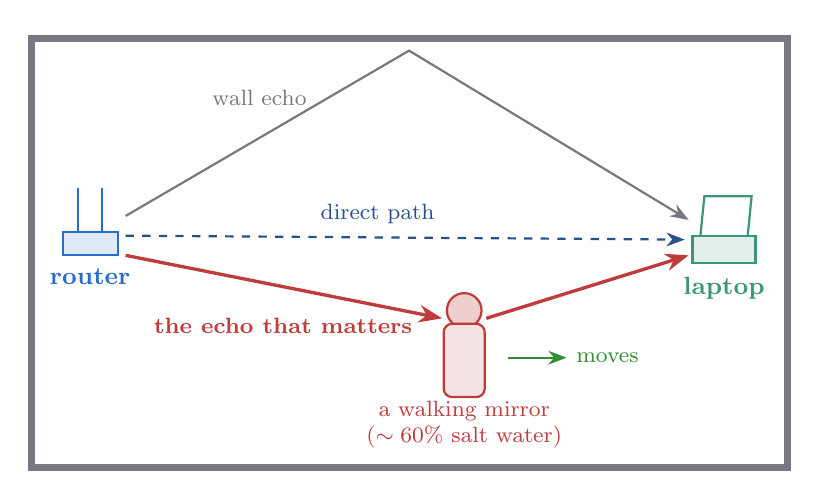
\begin{tikzpicture}[scale=1.0, >=Stealth]

  % Room walls
  \draw[wallgray, line width=2.5pt] (-4.8,-2.85) rectangle (4.8,2.6);

  % Router (TX) at left
  \draw[txcolor, thick, fill=txcolor!15] (-4.4,-0.15) rectangle (-3.7,0.15);
  \draw[txcolor, thick] (-4.2,0.15) -- (-4.2,0.7);
  \draw[txcolor, thick] (-3.9,0.15) -- (-3.9,0.7);
  \node[txcolor, font=\small\bfseries, below] at (-4.05,-0.2) {router};

  % Laptop (RX) at right
  \draw[rxcolor, thick, fill=rxcolor!15] (3.6,-0.25) rectangle (4.4,0.1);
  \draw[rxcolor, thick] (3.7,0.1) -- (3.75,0.6) -- (4.35,0.6) -- (4.3,0.1);
  \node[rxcolor, font=\small\bfseries, below] at (4.0,-0.3) {laptop};

  % Direct path
  \draw[accentblue, thick, dashed, ->] (-3.6,0.1) -- (3.5,0.05);
  \node[accentblue, font=\footnotesize, above] at (-0.4,0.12) {direct path};

  % Wall echo
  \draw[wallgray, thick, ->] (-3.6,0.35) -- (0,2.45) -- (3.55,0.3);
  \node[wallgray, font=\footnotesize, above] at (0,2.5) {};
  \node[wallgray, font=\footnotesize] at (-1.9,1.85) {wall echo};

  % Person
  \filldraw[personcolor!25, draw=personcolor, thick] (0.7,-0.85) circle (0.22);
  \draw[personcolor, thick, fill=personcolor!15, rounded corners=3pt] (0.44,-1.95) rectangle (0.96,-1.02);
  \node[personcolor, font=\footnotesize, align=center] at (0.7,-2.3) {a walking mirror\\($\sim 60\%$ salt water)};

  % Person echo
  \draw[personcolor, very thick, ->] (-3.6,-0.15) -- (0.42,-0.95);
  \draw[personcolor, very thick, ->] (0.98,-0.95) -- (3.55,-0.15);
  \node[personcolor, font=\footnotesize\bfseries] at (-1.6,-1.05) {the echo that matters};

  % Motion arrow
  \draw[arrowgreen, ->, thick] (1.25,-1.45) -- (2.0,-1.45);
  \node[arrowgreen, font=\footnotesize, right] at (2.0,-1.45) {moves};

\end{tikzpicture}
\caption{The receiver never hears one signal. It hears the direct path, the wall echoes, and the echo off the person, all added together into a single overlapping sum. Everything in this article comes from watching how that sum changes when one of the mirrors---the person---moves.}
\label{fig:room}
\end{figure}

Here's the part almost nobody knows: \textbf{your radio already measures this hall of mirrors, constantly, because it has to.} Overlapping echoes smear data---the wireless equivalent of trying to understand someone shouting in a cathedral. So before decoding anything, a modern Wi-Fi receiver first measures exactly how the room has distorted the signal, across dozens of frequencies, on every single packet, and then un-distorts it. Engineers call that measurement \textit{channel state information}. It is, quite literally, a running logbook of the room's echoes, updated hundreds of times per second.

To deliver your email at all, the radio must first measure the room. Sensing is nothing more than reading that measurement instead of throwing it away.

\subsection{Detection: when the mirror moves, the sum flickers}

What does ``the sum of all echoes'' actually do at the receiver? Waves add the way ripples on a pond add. If two echoes arrive \textit{in step}---crest lands on crest---they reinforce, and the signal is loud. If one echo has traveled just \textbf{half a wavelength} farther, crest lands on trough, and they cancel: quiet. In between, something in between.

\begin{figure}[ht]
\centering
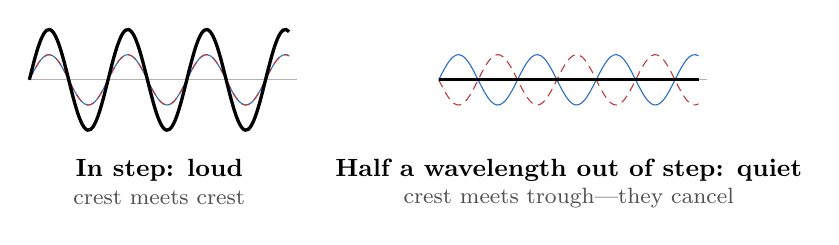
\begin{tikzpicture}[scale=1.0, >=Stealth]

  % ---------- Left panel: in phase ----------
  \begin{scope}[shift={(-4.3,0)}]
    \draw[gray!60] (0,0) -- (3.4,0);
    \draw[txcolor, thin] plot[domain=0:3.3, samples=90, smooth] (\x,{0.32*sin(360*\x)});
    \draw[personcolor, thin, densely dashed] plot[domain=0:3.3, samples=90, smooth] (\x,{0.32*sin(360*\x)});
    \draw[black, very thick] plot[domain=0:3.3, samples=90, smooth] (\x,{0.64*sin(360*\x)});
    \node[font=\small\bfseries] at (1.65,-1.15) {In step: loud};
    \node[font=\footnotesize, seriestitle] at (1.65,-1.5) {crest meets crest};
  \end{scope}

  % ---------- Right panel: half wavelength shift ----------
  \begin{scope}[shift={(0.9,0)}]
    \draw[gray!60] (0,0) -- (3.4,0);
    \draw[txcolor, thin] plot[domain=0:3.3, samples=90, smooth] (\x,{0.32*sin(360*\x)});
    \draw[personcolor, thin, densely dashed] plot[domain=0:3.3, samples=90, smooth] (\x,{0.32*sin(360*\x+180)});
    \draw[black, very thick] (0,0) -- (3.3,0);
    \node[font=\small\bfseries] at (1.65,-1.15) {Half a wavelength out of step: quiet};
    \node[font=\footnotesize, seriestitle] at (1.65,-1.5) {crest meets trough---they cancel};
  \end{scope}

\end{tikzpicture}
\caption{The whole game in one picture. Blue: an echo off the walls. Dashed red: the echo off the person. Black: what the receiver actually hears---their sum. Shift the red echo by a mere half wavelength (six centimeters at 2.4~GHz) and the sum flips from loud to quiet.}
\label{fig:superposition}
\end{figure}

Now let the person take a step. The echo bouncing off them gets a little longer or shorter---and remember, at Wi-Fi wavelengths, ``a little'' matters enormously. Move so that your echo's path changes by \textit{six centimeters}, and that echo swings all the way from reinforcing the others to canceling them. The received signal flickers.

So presence detection is almost embarrassingly easy. An empty room is a frozen hall of mirrors: the sum of echoes is rock steady, packet after packet. The moment anything alive moves---a step, a reach for the remote, a turn of the head---the sum trembles. The receiver doesn't need to know \textit{where} you are to know \textit{that} you are. Stillness has a signature, and you just broke it.

\subsection{Breathing: the slowest dance in the room}

Here's where it gets eerie. Suppose you sit perfectly still. Are you invisible now?

No---because you aren't actually still. Your chest rises and falls by roughly a centimeter with every breath. That motion stretches and shrinks your echo's path by a couple of centimeters, which at Wi-Fi wavelengths is a healthy fraction of a full wave. The result: the received signal strength doesn't just sit there---it \textit{sways}, gently, twelve to eighteen times per minute, perfectly in time with your lungs.

And that slow sway is absurdly easy to find, for one reason: \textbf{nothing else in a still room oscillates four times a minute.} Furniture doesn't breathe. Walls don't breathe. The radio samples the room hundreds of times per second, so a four-second rhythm is, to it, glacial---trivial to average out of the noise. Your router's signal meter is quietly rocking back and forth with your chest, and it has been since the day you plugged it in.

\subsection{Where you are: rings of loud and quiet}

Detection is one thing. \textit{Location} needs geometry---and the geometry here is genuinely beautiful.

Ask: at which spots in the room would a person's echo arrive exactly in step with the direct signal? Answer: all the places where the detour path (router~$\to$~person~$\to$~laptop) exceeds the direct path by a whole number of wavelengths. Those places form nested \textbf{ellipse-shaped rings} around the line between router and laptop---like the layers of an onion, with the two radios buried inside. In one ring your echo reinforces; in the next ring out, it cancels; then reinforces again. Rings of loud and quiet, tens of centimeters apart, invisibly tiling your living room.

\begin{figure}[ht]
\centering
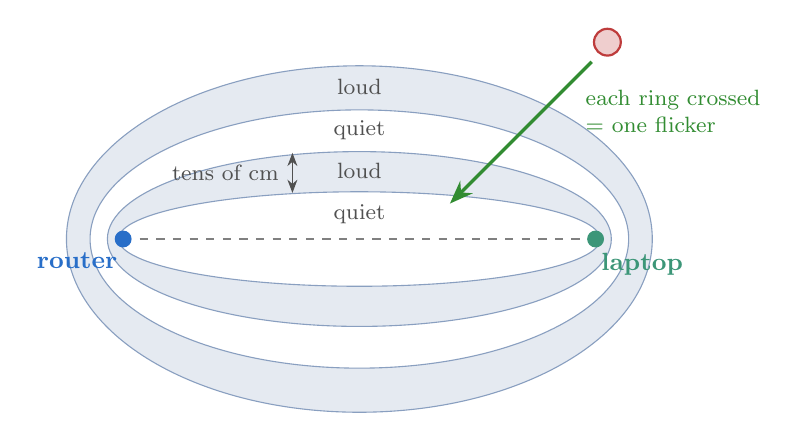
\begin{tikzpicture}[scale=1.0, >=Stealth]

  % Alternating zone fills, outermost first
  \fill[accentblue!12] (0,0) ellipse (3.72 and 2.20);
  \fill[white]         (0,0) ellipse (3.42 and 1.64);
  \fill[accentblue!12] (0,0) ellipse (3.20 and 1.11);
  \fill[white]         (0,0) ellipse (3.06 and 0.60);

  % Zone boundaries
  \draw[accentblue!55, thin] (0,0) ellipse (3.72 and 2.20);
  \draw[accentblue!55, thin] (0,0) ellipse (3.42 and 1.64);
  \draw[accentblue!55, thin] (0,0) ellipse (3.20 and 1.11);
  \draw[accentblue!55, thin] (0,0) ellipse (3.06 and 0.60);

  % Direct line between foci
  \draw[gray, dashed] (-3,0) -- (3,0);

  % TX and RX at the foci
  \filldraw[txcolor] (-3,0) circle (0.10);
  \node[txcolor, font=\small\bfseries, below left] at (-2.95,-0.05) {router};
  \filldraw[rxcolor] (3,0) circle (0.10);
  \node[rxcolor, font=\small\bfseries, below right] at (2.95,-0.05) {laptop};

  % loud / quiet labels up the vertical axis
  \node[font=\footnotesize, seriestitle] at (0,0.32) {quiet};
  \node[font=\footnotesize, seriestitle] at (0,0.86) {loud};
  \node[font=\footnotesize, seriestitle] at (0,1.38) {quiet};
  \node[font=\footnotesize, seriestitle] at (0,1.93) {loud};

  % ring spacing annotation
  \draw[seriestitle, <->, thin] (-0.85,0.585) -- (-0.85,1.095);
  \node[seriestitle, font=\footnotesize, left] at (-0.9,0.84) {tens of cm};

  % Person crossing the rings
  \filldraw[personcolor!25, draw=personcolor, thick] (3.15,2.5) circle (0.17);
  \draw[arrowgreen, very thick, ->] (2.95,2.25) -- (1.15,0.45);
  \node[arrowgreen, font=\footnotesize, right, align=left] at (2.75,1.62) {each ring crossed\\= one flicker};

\end{tikzpicture}
\caption{The interference rings (physicists call them Fresnel zones) around a router--laptop pair. Inside each ring, the echo off a person adds in step with the direct signal; in the next ring, out of step. Walk across the rings and the received signal blinks once per ring---so the blink rate reveals your speed, and the character of each blink reveals your direction.}
\label{fig:fresnel}
\end{figure}

Now everything clicks into place:

\begin{itemize}[nosep]
  \item \textbf{Speed.} Walk across the rings and the signal blinks once per ring crossed. Blink faster, you're moving faster. At a normal walking pace this is a flutter of roughly ten to thirty blinks per second---unmistakable.
  \item \textbf{Direction.} Each blink also carries a subtle ``handedness''---the echo drifts through its cycle one way when your path is shrinking and the opposite way when it's growing. Toward the kitchen and away from it produce mirror-image flickers.
  \item \textbf{Place.} One router--laptop pair gives you one family of rings. But your home has many pairs: router to laptop, router to phone, router to TV, node to node in a mesh. Each pair lays down its own onion of rings at its own angle, and a person stands at the \textit{intersection} of whichever rings they're disturbing. More pairs, tighter intersection, better fix. And routers with several antennas add one more trick: like a pair of ears, two antennas hear the same echo at minutely different moments, which reveals the \textit{direction} it came from.
\end{itemize}

\subsection{Through the wall}

One loose end: claim number one said \textit{through a wall}. But there's nothing left to explain---you already know Wi-Fi passes through interior walls, because you use it in the next room every day. At these wavelengths drywall is frosted glass: the light gets through, merely dimmed. So the hall of mirrors doesn't end at the wall, and neither does the flicker of a person moving behind it. The picture is fainter, blurrier---but it's there. (Thick poured concrete, on the other hand, is more like a welding mask, which is also why your signal dies in the basement stairwell. The limits of your network's reach and the limits of its vision are the same limits.)

\subsection{The complete picture}

Without a single equation, one idea---\textit{the receiver hears every echo added together, and you are one of the echoes}---has delivered all four claims:

\begin{itemize}[nosep]
  \item \textbf{Presence} is any tremble at all in an otherwise frozen sum of echoes---even through drywall.
  \item \textbf{Breathing} is the slow, four-second sway of one echo's path, unmistakable because nothing else in the room moves that slowly and steadily.
  \item \textbf{Motion and direction} come from crossing the rings of loud and quiet: blink rate is speed, blink handedness is direction.
  \item \textbf{Location and pose} come from stacking many router--device pairs and many antennas, each contributing its own rings and bearings, until the intersections sketch a silhouette.
\end{itemize}

The lesson, which we'll widen at the end, is this: \textit{a wave that carries a message also carries a map.} Every path it takes leaves a fingerprint on it. Your Wi-Fi was never just delivering email; it was surveying the house the whole time.

% ================================================================
% PART 2
% ================================================================

\section{The Physics, Made Rigorous}

Time to justify the hand-waving. Everything in Part~1 rests on three claims: that your body reflects Wi-Fi strongly, that the receiver measures a coherent sum of echoes, and that tiny motions produce large, structured changes in that sum. Let's prove each, with numbers.

\subsection{The wave, the room, and the channel}

Wi-Fi operates near $f = 2.4$, $5$, and $6\ \text{GHz}$, so the wavelengths are
\begin{equation}
  \lambda = \frac{c}{f}: \qquad
  \lambda_{2.4\,\text{GHz}} \approx 12.5\ \text{cm}, \qquad
  \lambda_{5\,\text{GHz}} \approx 6.0\ \text{cm}, \qquad
  \lambda_{6\,\text{GHz}} \approx 5.0\ \text{cm}.
\end{equation}
Centimeter-scale wavelengths are the size regime of human motion---which is the deep reason Wi-Fi sensing works at all.

In a multipath environment, the channel between transmitter and receiver is the coherent sum over all propagation paths $k$, each with amplitude $a_k$ and delay $\tau_k = d_k/c$:
\begin{equation}
  H(f, t) \;=\; \sum_k a_k(t)\, e^{-j 2\pi f \tau_k(t)} .
  \label{eq:channel}
\end{equation}
This complex number $H$---one per frequency---is exactly the ``sum of echoes'' of Part~1, amplitude \textit{and} phase.

And here is the engineering fact that makes everything practical: Wi-Fi is an OFDM system. It splits its band into dozens to hundreds of narrow subcarriers, and to equalize the link the receiver \textit{estimates $H$ on every subcarrier of every packet}---this is the channel state information (CSI) mentioned in Part~1. A commodity chipset therefore produces hundreds of complex samples of equation~\eqref{eq:channel}, refreshed as fast as packets fly, typically hundreds of times per second. Not a one-pixel camera after all: a few hundred one-pixel cameras, at different colors of radio light, blinking hundreds of times a second. Sensing algorithms simply read this stream.

\subsection{Why the body reflects: the dielectrics of salt water}

At microwave frequencies, tissue behaves as a lossy dielectric with complex relative permittivity $\varepsilon_r = \varepsilon' - j\varepsilon''$, where $\varepsilon'' = \sigma/(\omega \varepsilon_0)$ captures conductive and dipolar losses. Measured values for muscle at $2.45\ \text{GHz}$ are approximately $\varepsilon' \approx 53$ and $\sigma \approx 1.7\ \text{S/m}$, giving
\begin{equation}
  \varepsilon_r \;\approx\; 53 - 13j .
\end{equation}
For a wave in air striking this medium at normal incidence, the amplitude reflection coefficient is
\begin{equation}
  \Gamma \;=\; \frac{1 - \sqrt{\varepsilon_r}}{1 + \sqrt{\varepsilon_r}}, \qquad
  |\Gamma| \approx 0.76, \qquad |\Gamma|^2 \approx 0.58 .
\end{equation}
So roughly \textbf{60\% of the incident power reflects straight off the skin}---the ``wet mirror'' of Part~1, now quantified. The transmitted remainder decays with a penetration depth of about $2\ \text{cm}$ in muscle at these frequencies, so the body is optically thick: nothing passes through, and the echo comes from the surface. Overall, a standing adult presents a radar cross-section of order $0.1$--$1\ \text{m}^2$, comparable to a small metal panel.

(The power numbers behind Part~1's reassurance: a router transmits on the order of $100\ \text{mW}$, spread over the house and mostly missing you; your basal metabolism runs at about $100\ \text{W}$. Even total absorption of the router's entire output would add $\sim 0.1\%$ to your own internal heating. The physics that lets Wi-Fi \textit{see} you involves microwatts of reflected power, not heating.)

While we're here, the wall claim: at these frequencies a sheet of drywall typically costs a wave a few dB per pass, while thick poured or reinforced concrete costs tens of dB. That single fact sets both the range of your network and the range of its vision.

\subsection{How big is the echo?}

Before celebrating, we should worry. The echo off a person is weak. Compare the direct path (length $d$) with the reflected path (transmitter to person, $d_1$; person to receiver, $d_2$; radar cross-section $\sigma$). The Friis and bistatic-radar equations give
\begin{equation}
  \frac{P_{\text{echo}}}{P_{\text{direct}}}
  \;=\; \frac{\sigma\, d^2}{4\pi\, d_1^2\, d_2^2} .
\end{equation}
Put in living-room numbers: $d = 5\ \text{m}$, $d_1 = d_2 = 3\ \text{m}$, $\sigma = 0.3\ \text{m}^2$:
\begin{equation}
  \frac{P_{\text{echo}}}{P_{\text{direct}}} \;\approx\; \frac{0.3 \times 25}{4\pi \times 81}
  \;\approx\; 7\times 10^{-3} \quad (\approx -21\ \text{dB}).
\end{equation}
The person's echo carries \textbf{less than 1\% of the power} of the direct signal. Naively, moving a mirror that faint should change the received power by less than 1\%---down in the noise. So why does any of this work?

\subsection{The absurd twist: interference is an amplifier}

Here is the gem of this episode.

Split the channel into the static room (walls, floor, furniture---call their combined echo $\Hs$) plus the one dynamic echo off the person, whose path length $d_p(t)$ changes as they move:
\begin{equation}
  H(t) \;=\; \Hs \;+\; a\, e^{-j 2\pi d_p(t)/\lambda},
  \qquad \text{with } \epsilon \equiv \frac{|a|}{|\Hs|} \approx \sqrt{7\times10^{-3}} \approx 0.09 .
\end{equation}
The receiver measures power:
\begin{equation}
  |H|^2 \;=\; |\Hs|^2 \Big( 1 + \epsilon^2 + 2\epsilon \cos\phi(t) \Big),
  \qquad \phi(t) = \frac{2\pi\, d_p(t)}{\lambda} + \text{const}.
  \label{eq:crossterm}
\end{equation}
Look at the two person-dependent terms. The echo's own power, $\epsilon^2 \approx 0.008$, is indeed invisible. But the \textbf{cross term} $2\epsilon\cos\phi$ swings the total received power by $\pm 2\epsilon \approx \pm 18\%$. Interference has amplified the visibility of the echo by a factor of $2\epsilon / \epsilon^2 = 2/\epsilon \approx 23$.

This is worth staring at. Interference responds to the echo's \textit{amplitude} ($\epsilon$), not its \textit{power} ($\epsilon^2$)---the big static echo acts as a built-in reference beam that beats against the faint moving one. And the fainter the echo, the \textit{larger} the amplification factor $2/\epsilon$ becomes. A sub-1\%-power echo produces a nearly 20\% swing in what the receiver measures. The hall of mirrors isn't an obstacle to sensing; it is the instrument. (Readers who know optics will recognize this as homodyne detection---the same trick behind holography and LIGO---happening by accident in your hallway.)

\begin{figure}[ht]
\centering
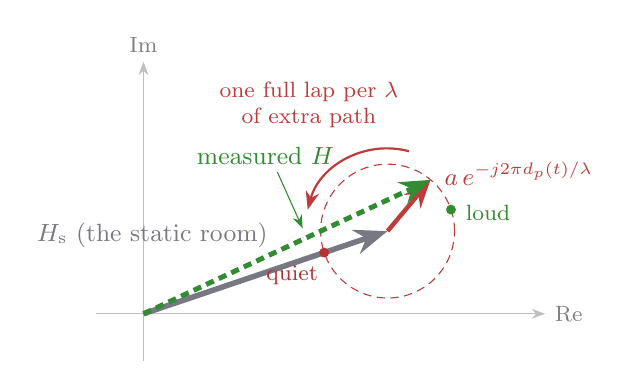
\begin{tikzpicture}[scale=1.0, >=Stealth]

  % axes
  \draw[gray!50, ->] (-0.6,0) -- (5.1,0) node[right, gray, font=\footnotesize] {Re};
  \draw[gray!50, ->] (0,-0.6) -- (0,3.2) node[above, gray, font=\footnotesize] {Im};

  % static channel vector
  \draw[wallgray, line width=2pt, ->] (0,0) -- (3.1,1.05);
  \node[wallgray, font=\small, above left] at (1.7,0.72) {$\Hs$ (the static room)};

  % circle traced by the tip
  \draw[personcolor, densely dashed] (3.1,1.05) circle (0.85);

  % person's echo vector
  \draw[personcolor, line width=1.6pt, ->] (3.1,1.05) -- (3.646,1.701);
  \node[personcolor, font=\small, right] at (3.7,1.78) {$a\,e^{-j 2\pi d_p(t)/\lambda}$};

  % resultant
  \draw[arrowgreen, line width=1.8pt, densely dashed, ->] (0,0) -- (3.646,1.701);
  \node[arrowgreen, font=\small] at (1.55,2.0) {measured $H$};
  \draw[arrowgreen, thin, ->, shorten >=2pt] (1.7,1.8) -- (2.05,1.02);

  % rotation arrow
  \draw[personcolor, ->, thick] ([shift={(75:1.05)}]3.1,1.05) arc[start angle=75, end angle=165, radius=1.05];
  \node[personcolor, font=\footnotesize, align=center] at (2.1,2.65) {one full lap per $\lambda$\\ of extra path};

  % loud / quiet points on the circle
  \filldraw[arrowgreen] (3.905,1.323) circle (0.055);
  \node[arrowgreen, font=\footnotesize, right] at (3.97,1.28) {loud};
  \filldraw[arrowred] (2.295,0.777) circle (0.055);
  \node[arrowred, font=\footnotesize, below left] at (2.34,0.74) {quiet};

\end{tikzpicture}
\caption{The channel as a clock. The long hand $\Hs$ is the frozen sum of all static echoes. The short hand is the person's echo: as they move, it spins---one full revolution for each wavelength of change in their echo path. The receiver measures the total hand $H$, whose length breathes between ``loud'' and ``quiet.'' Though the short hand carries under 1\% of the power, it swings the measured power by nearly 20\%, because interference responds to amplitude, not power.}
\label{fig:phasor}
\end{figure}

\subsection{Breathing, quantitatively}

Quiet breathing moves the chest wall by $\Delta x \approx 0.5\ \text{cm}$. For an echo that goes out and back off the chest, the path length changes by about $2\Delta x$, so the phase in equation~\eqref{eq:crossterm} sways by
\begin{equation}
  \Delta\phi \;=\; \frac{4\pi\, \Delta x}{\lambda}
  \;\approx\; 60^\circ \ \text{at } 5\ \text{GHz}, \qquad 29^\circ \ \text{at } 2.4\ \text{GHz}.
\end{equation}
A $60^\circ$ sweep of the cross term moves the received power by several percent---sitting on a carrier of $0.2$--$0.3\ \text{Hz}$ (12--18 breaths per minute). Since CSI is sampled at hundreds of hertz, one narrow band-pass filter around $0.1$--$0.5\ \text{Hz}$ plus a minute of averaging pulls the breathing waveform cleanly out of the noise. (One honest subtlety: the sensitivity $\partial |H|^2 / \partial d_p$ depends on where you sit in $\phi$---mid-ring versus ring boundary in Figure~\ref{fig:fresnel}---which is exactly why real systems find breathing easier to read from some couch positions than others. The Fresnel geometry isn't decoration; it's the operating manual.)

\subsection{Walking: fringes, Doppler, and direction}

A person walking changes $d_p(t)$ at up to twice their speed $v$ (path out \textit{and} path back both shrink when you walk straight at the link). Equation~\eqref{eq:crossterm} then oscillates at the fringe rate
\begin{equation}
  f_{\text{fringe}} \;=\; \frac{1}{\lambda}\left|\frac{\mathrm{d} d_p}{\mathrm{d}t}\right| \;\le\; \frac{2v}{\lambda}
  \;\approx\; 16\ \text{Hz at } v = 1\ \tfrac{\text{m}}{\text{s}},\ 2.4\ \text{GHz}.
\end{equation}
This is the blink-per-ring-crossed of Part~1, and it is also a Doppler shift in disguise: the moving body shifts its echo's frequency by $f_{\text{fringe}}$, and that shifted echo \textit{beats} against the static room at the difference frequency. Note the absurdity of the scale: $16\ \text{Hz}$ against a $2.4\ \text{GHz}$ carrier is a fractional shift of $7\times 10^{-9}$---seven parts per billion, hopeless to measure as a frequency change. Interference converts it into a large, slow, visible flutter for free. Direction comes along too: the sign of $\mathrm{d}d_p/\mathrm{d}t$ sets the rotation sense of the short hand in Figure~\ref{fig:phasor}---counterclockwise approaching, clockwise receding---so approach and retreat are mirror-image signatures, just as Part~1 promised.

\subsection{Location: three coordinates, three tricks}

\subsubsection{Trick 1: the rings, derived}

A point at perpendicular distance $r$ from the router--laptop line, at distances $d_1$ and $d_2$ from the two radios along it, adds excess path length $\Delta\ell$ (bounced route minus direct route):
\begin{equation}
  \Delta\ell \;=\; \sqrt{d_1^2 + r^2} + \sqrt{d_2^2 + r^2} - (d_1 + d_2)
  \;\approx\; \frac{r^2}{2}\left(\frac{1}{d_1} + \frac{1}{d_2}\right)
  \quad (r \ll d_1, d_2).
\end{equation}
Each half wavelength of extra path slips the echo's phase by $\pi$ relative to the direct signal---one flip between reinforcing and canceling---so setting $\Delta\ell = n\lambda/2$ gives the ring boundaries of Figure~\ref{fig:fresnel}:
\begin{equation}
  r_n \;=\; \sqrt{\frac{n\,\lambda\, d_1 d_2}{d_1 + d_2}} .
\end{equation}
For a router and laptop $6\ \text{m}$ apart at $2.4\ \text{GHz}$, midway between them: $r_1 \approx 43\ \text{cm}$, $r_2 \approx 61\ \text{cm}$, $r_3 \approx 75\ \text{cm}$---boundaries roughly $15$--$20\ \text{cm}$ apart, tightening outward. Crossing them at walking pace reproduces the fringe rates above: the Doppler picture and the ring picture are the same physics in different clothes.

\subsubsection{Trick 2: bearing from an antenna array}

Two antennas spaced $d$ apart receive the same echo with a path difference $d\sin\theta$, hence a phase difference
\begin{equation}
  \Delta\phi \;=\; \frac{2\pi d}{\lambda}\, \sin\theta ,
\end{equation}
where $\theta$ is the arrival angle. This is precisely how your two ears localize sound. A MIMO router carries two to eight antennas for data throughput---and the identical hardware, read as phases, becomes a direction finder.

\subsubsection{Trick 3: range from bandwidth}

Echo \textit{delay} separates targets by distance, but only as sharply as the bandwidth $B$ allows: two echoes blur together unless their round-trip paths differ by more than
\begin{equation}
  \Delta d \;=\; \frac{c}{2B} .
\end{equation}

\begin{figure}[ht]
\centering
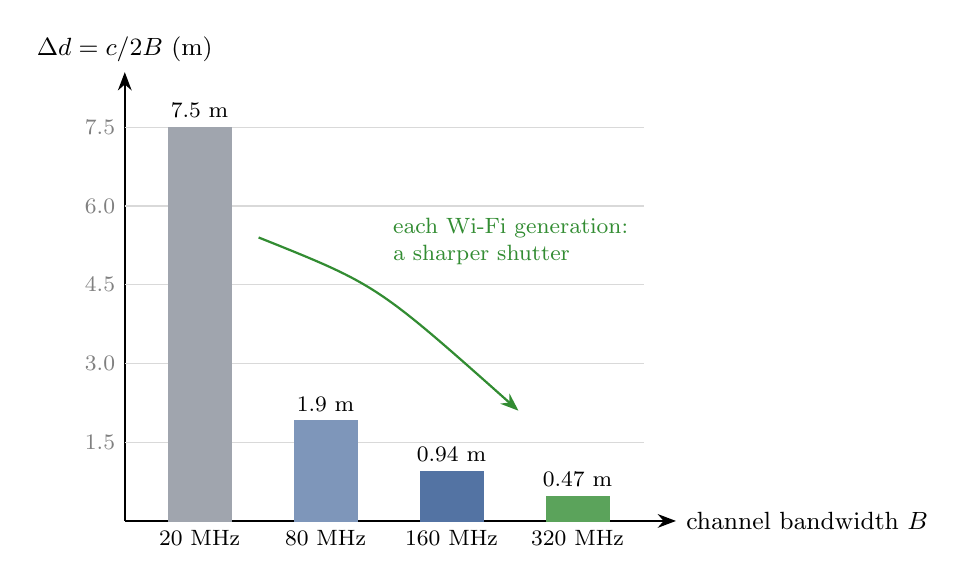
\begin{tikzpicture}[scale=1.0, >=Stealth]
  % axes
  \draw[->, thick] (0,0) -- (0,5.7) node[above, font=\small] {$\Delta d = c/2B$ (m)};
  \draw[->, thick] (0,0) -- (7.0,0) node[right, font=\small] {channel bandwidth $B$};

  % gridlines: 1 unit = 1.5 m
  \foreach \v/\h in {1.5/1.0, 3.0/2.0, 4.5/3.0, 6.0/4.0, 7.5/5.0} {
    \draw[gray!30] (0,\h) -- (6.6,\h);
    \node[left, font=\footnotesize, gray] at (0,\h) {\v};
  }

  % bars
  \filldraw[quietgray!90] (0.55,0) rectangle (1.35,5.0);
  \node[above, font=\footnotesize] at (0.95,5.0) {$7.5$ m};
  \node[below, font=\footnotesize] at (0.95,0) {$20$ MHz};

  \filldraw[accentblue!60] (2.15,0) rectangle (2.95,1.27);
  \node[above, font=\footnotesize] at (2.55,1.27) {$1.9$ m};
  \node[below, font=\footnotesize] at (2.55,0) {$80$ MHz};

  \filldraw[accentblue!80] (3.75,0) rectangle (4.55,0.63);
  \node[above, font=\footnotesize] at (4.15,0.63) {$0.94$ m};
  \node[below, font=\footnotesize] at (4.15,0) {$160$ MHz};

  \filldraw[arrowgreen!80] (5.35,0) rectangle (6.15,0.31);
  \node[above, font=\footnotesize] at (5.75,0.31) {$0.47$ m};
  \node[below, font=\footnotesize] at (5.75,0) {$320$ MHz};

  % annotation
  \draw[arrowgreen, thick, ->] (1.7,3.6) .. controls (3.2,3.0) .. (5.0,1.4);
  \node[arrowgreen, font=\footnotesize, align=left] at (4.9,3.55) {each Wi-Fi generation:\\ a sharper shutter};

\end{tikzpicture}
\caption{Range resolution versus channel bandwidth, $\Delta d = c/2B$. Early 20~MHz Wi-Fi could barely separate ``in this room'' from ``in that room''; the 320~MHz channels of Wi-Fi~7 resolve echoes to about half a meter. Bandwidth, added purely for faster downloads, doubles as the focus knob of the accidental radar.}
\label{fig:bandwidth}
\end{figure}

Notice what happened across Wi-Fi's history without anyone aiming for it: every upgrade made for \textit{communication} sharpened the \textit{sensor}. More bandwidth for throughput $\to$ finer range resolution. More antennas for MIMO capacity $\to$ finer bearing resolution. More devices per home $\to$ more ring families to intersect. Stack all three---delay, bearing, and multiple links---and you localize a moving person to well under a meter; push to research-grade arrays and processing, and the intersections sketch the coarse pose of a body, wall or no wall. The IEEE is now folding this in deliberately: the 802.11bf (``WLAN Sensing'') effort exists to standardize exactly these measurements. The accidental radar is being made official.

\subsection{Summary: one radio, many senses}

\begin{table}[H]
\centering
\renewcommand{\arraystretch}{1.35}
\begin{tabular}{@{}>{\raggedright}p{2.5cm} p{3.6cm} p{3.3cm} p{3.6cm}@{}}
\toprule
\textbf{What you learn} & \textbf{The measurement} & \textbf{Governing relation} & \textbf{Typical scale} \\
\midrule
Presence & any tremble in the frozen sum $H$ & eq.~\eqref{eq:crossterm} & the free byproduct \\
Breathing & slow sway of one echo's phase & $\Delta\phi = 4\pi\Delta x/\lambda$ & $\sim 60^\circ$ per breath at 5 GHz \\
Speed \& direction & fringe rate; rotation sense of the phasor & $f_{\text{fringe}} \le 2v/\lambda$ & $\sim 16$ Hz at walking pace \\
Bearing & phase across antennas & $\Delta\phi = \tfrac{2\pi d}{\lambda}\sin\theta$ & a router's 2--8 antennas \\
Range & echo delay vs.\ bandwidth & $\Delta d = c/(2B)$ & $7.5\ \text{m} \to 0.5\ \text{m}$ \\
\bottomrule
\end{tabular}
\caption{The senses of a Wi-Fi radio. Every row is extracted from the same stream of channel measurements the radio must make anyway to deliver data. Not one requires hardware that wasn't already there for communication.}
\label{tab:summary}
\end{table}

% ================================================================
% CLOSING
% ================================================================

\section*{Closing Thoughts}

Wi-Fi sensing is a dramatic case, but it is not a special one. The underlying principle is completely general: \textit{a wave that fills a space carries a map of that space}, because every reflection, every detour, every absorption leaves a fingerprint in its phase and amplitude. We usually treat waves as messengers and throw the fingerprints away. Reading them instead is a superpower we keep rediscovering.

Bats and submarines read the fingerprints in sound. Seismologists read earthquake waves that have passed through the planet, and from their echoes mapped Earth's liquid outer core---an image of a place no probe will ever visit. Physicists have read cosmic-ray muons passing through the Great Pyramid and found hidden voids in the stone. LIGO reads kilometer-scale interference fringes to catch spacetime itself stretching by less than a proton's width. Different waves, different rooms, one idea: the medium remembers where it has been, and interference is how you get it to talk.

There is an uncomfortable edge here, and it deserves a sentence in plain language: walls have always given us privacy from \textit{eyes}, and it is strange to learn they never gave us privacy from Maxwell's equations. The physics is indifferent to intent---the same flicker that lets a router notice a burglar lets it notice you, and the engineers standardizing Wi-Fi sensing are, to their credit, wrestling with that openly. The hopeful side of the ledger is real, too: a sensor that detects a grandparent's fall, or the breathing of someone trapped under rubble, without a single camera in the house, is a genuinely humane machine.

You might expect the truly strange physics to live in exotic, faraway places. Episode after episode, the lesson is the opposite. The ordinary world is already absurd: the little blinking box in your hallway has been painting the room in invisible centimeter-long light, and reading the reflections off your body, since the day you plugged it in---then politely discarding the picture to bring you your email. The picture was always there. You just have to know how to read it.

\vspace{1cm}
\begin{center}
\rule{0.4\textwidth}{0.5pt}
\end{center}

\vspace{1cm}

\subsection*{A Note on Accuracy}

Tissue dielectric values ($\varepsilon' \approx 53$, $\sigma \approx 1.7\ \text{S/m}$ for muscle at 2.45~GHz, penetration depth $\sim 2$~cm) are from the standard Gabriel measurements [2]; they vary by tissue type and person, and ``roughly 60\% of power reflects'' should be read as the right order of magnitude, not a universal constant. Fringe rates, phase swings, echo budgets, and ring spacings are computed for representative living-room geometries and scale with the actual distances, wavelength, and posture involved. Wall attenuations (``a few dB'' for drywall, ``tens of dB'' for thick concrete) are typical ranges, not specifications. On capability tiers: presence, motion, and breathing detection are demonstrated on commodity Wi-Fi hardware and, in the case of motion sensing, sold as a consumer feature; through-wall pose reconstruction [4, 5, 6] has been achieved with purpose-built multi-antenna radio arrays and, more recently and more coarsely, with commodity Wi-Fi chipsets plus substantial machine-learning processing---it is not a firmware toggle on a stock router. Household Wi-Fi power levels are non-ionizing and far below thermal significance, as estimated in Part~2. Nothing in this article is a how-to; it is an explanation of physics that the research community has published openly and that standards bodies [8] are now engineering deliberately, privacy safeguards included.

\subsection*{References}

\begin{enumerate}[label={[\arabic*]}, leftmargin=*, itemsep=2pt]
  \item Griffiths, D.~J., \textit{Introduction to Electrodynamics}, 4th ed. Cambridge University Press, 2017. (Electromagnetic waves, reflection at interfaces, and the interference arguments used throughout the \seriesname{} series.)
  \item Gabriel, S., Lau, R.~W., and Gabriel, C., ``The dielectric properties of biological tissues: II. Measurements in the frequency range 10~Hz to 20~GHz,'' \textit{Physics in Medicine and Biology}, vol.~41, no.~11, pp.~2251--2269, 1996. \texttt{doi:10.1088/0031-9155/41/11/002}.
  \item Halperin, D., Hu, W., Sheth, A., and Wetherall, D., ``Tool Release: Gathering 802.11n Traces with Channel State Information,'' \textit{ACM SIGCOMM Computer Communication Review}, vol.~41, no.~1, p.~53, 2011. \texttt{doi:10.1145/1925861.1925870}. (The measurement tool that opened commodity CSI to researchers.)
  \item Adib, F. and Katabi, D., ``See Through Walls with WiFi!,'' \textit{Proceedings of ACM SIGCOMM}, pp.~75--86, 2013. \texttt{doi:10.1145/2486001.2486039}.
  \item Zhao, M., Li, T., Abu Alsheikh, M., Tian, Y., Zhao, H., Torralba, A., and Katabi, D., ``Through-Wall Human Pose Estimation Using Radio Signals,'' \textit{Proceedings of IEEE CVPR}, pp.~7356--7365, 2018.
  \item Geng, J., Huang, D., and De~la~Torre, F., ``DensePose From WiFi,'' \texttt{arXiv:2301.00250}, 2023. (Coarse body-pose estimation from commodity Wi-Fi hardware.)
  \item Ma, Y., Zhou, G., and Wang, S., ``WiFi Sensing with Channel State Information: A Survey,'' \textit{ACM Computing Surveys}, vol.~52, no.~3, art.~46, 2019. \texttt{doi:10.1145/3310194}.
  \item Du, R., Hua, H., Xie, H., et al., ``An Overview on IEEE 802.11bf: WLAN Sensing,'' \texttt{arXiv:2310.17661}, 2023. (The standardization effort to make Wi-Fi sensing an official part of the protocol.)
\end{enumerate}

\end{document}
